%! Author = user
%! Date = 3/9/2024

% Preamble
\documentclass{article}
\usepackage[utf8]{inputenc}
\usepackage{amsmath, amssymb, amsthm}
\usepackage{tikz}
\usepackage{pgfplots}
\usepackage{subfigure}
\usepackage{listings}
\usepackage[fontsize=13.5pt]{fontsize}
\usepackage[a4paper,
            bindingoffset=.2in,
            left=.7in,
            right=.7in,
            top=1in,
            bottom=1in,
            footskip=.25in]{geometry}

\definecolor{dkgreen}{rgb}{0,0.6,0}
\definecolor{gray}{rgb}{0.5,0.5,0.5}
\definecolor{mauve}{rgb}{0.58,0,0.82}

\lstset{frame=tb,
  language=Java,
  aboveskip=3mm,
  belowskip=3mm,
  showstringspaces=false,
  columns=flexible,
  basicstyle={\small\ttfamily},
  numbers=none,
  numberstyle=\tiny\color{gray},
  keywordstyle=\color{blue},
  commentstyle=\color{dkgreen},
  stringstyle=\color{mauve},
  breaklines=true,
  breakatwhitespace=true,
  tabsize=3
}

\title{LaTex for Students}
\author{Jun Ho Lee}
\date{March 2024}

% Document
\begin{document}

\newpage
\section{Week4}

Deep Neural Network.

\subsection{Depp L-layer Neural Network}


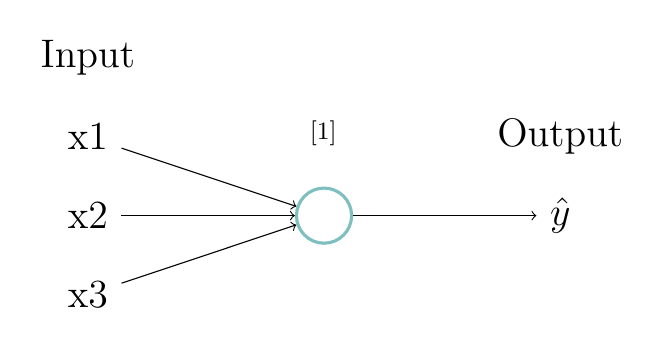
\begin{tikzpicture}
    % Input Layer
    \foreach \name/\i in {x1/1,x2/2,x3/3} {
        \node (Input-\i) at (0,-\i) {\name};
        \ifnum \i=1
            \node[above of=Input-\i] {Input};
        \fi
    }
    % Hidden Layer
    \foreach \i in {1} {
        \node[circle, minimum size = 7mm, draw=teal!50, line width=.4mm] (Hidden1-\i) at (3,-2) {};
        \ifnum \i=1
        \node[above of=Hidden1-\i] {$^{[1]}$};
        \fi
    }
    % Output Layer
    \foreach \name/\i in {$\hat{y}$/1} {
        \node (Output-\i) at (6,-2) {\name};
        \ifnum \i=1
        \node[above of=Output-\i] {Output};
        \fi
    }
    % Arrows
    \foreach \i in {1,2,3} {
        \foreach \j in {1} {
           \draw[->] (Input-\i) -- (Hidden1-\j);
        }
    }
    \foreach \i in {1} {
        \foreach \j in {1} { \draw[->] (Hidden1-\i) -- (Output-\j);
        }
    }
\end{tikzpicture}


\end{document}

